\documentclass{./../div_teaching_slides}
\begin{document}

\title{ECON 340 \\ Economic Research Methods}
\author{Div Bhagia}
\date{Lecture 1: Introduction}

\begin{frame}[noframenumbering, plain]
\maketitle
\end{frame}


\begin{frame}{So many questions...}
Always have questions that need answers \\ \vskip0.25em
\begin{witemize}
\item Do electric vehicle subsidies increase sales? 
\item Does the use of phones inhibit classroom learning?
\item Is there racial discrimination in the labor market?
\item Does raising interest rates lead to inflation?
\item Who will win the next US election? 
\end{witemize}
\vspace{0.75em}
\end{frame}

\begin{frame}{Quantitive Empirical Research}
\begin{witemize}
  \item A \textit{research question} is any question you plan to answer by conducting research
  \item \textit{Empirical research} is based on real-world observations
  \item \textit{Quantitative empirical research}: empirical research that uses quantitative measurements
  \item In this class, we will learn to answer a research question using quantitative empirical research 
\end{witemize}
\end{frame}

\begin{frame}{Quantitive Empirical Research}
Everyone is using it (for good reason) \\
\begin{witemize}
\item Economists, other social scientists
\item Think tanks, governments, policymakers 
\item Businesses 
\end{witemize}
Our world is becoming more and more data-oriented.
\end{frame}

\begin{frame}{Most used words in economic papers}
\vspace{1.5em}
\begin{columns}
\begin{column}[c]{0.3\textwidth}
\centering
\purple{1970s} \\ \vspace{0.75em}
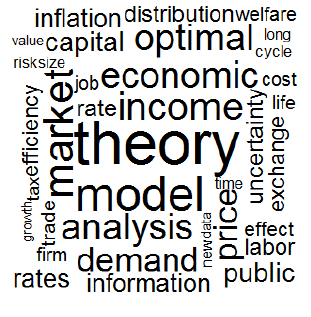
\includegraphics[scale=0.4]{1970.png}
\end{column}
\begin{column}[c]{0.3\textwidth}
\centering
\purple{1990s} \\ \vspace{0.75em}

\includegraphics[scale=0.4]{1990.png}
\end{column}
\begin{column}[c]{0.3\textwidth}
\centering
\purple{2010-2015} \\ \vspace{0.75em}

\includegraphics[scale=0.4]{2010.png}
\end{column}
\end{columns}
\end{frame}


\begin{frame}{This Course}
Introduce you to tools used in quantitative research \\~\\
Main goals:\\
\begin{witemize}
\item Understand statistical and econometric methods
\item Be able to implement these methods in R
\item Carry out a research project
\end{witemize}
\end{frame}

%\begin{frame}{Topics Covered}
%\begin{witemize}
%\item How to write a research paper? What's a good research question? Where to find data?
%\item Summarizing data using distributions, mean, variance, correlation, etc.
%\item Random sampling and inference in the face of uncertainty (confidence intervals, hypothesis testing)
%\item Using the Linear Regression Model (LRM) for prediction and causal inference
%\end{witemize}
%\end{frame}

\begin{frame}{Course Components}
\begin{witemize}
\item Active Engagement (10\%)
\item Problem Sets (20\%)
\item Research Paper: Interim Submissions (15\%)
\item Research Paper: Final Submissions (15\%)
\item Midterm (20\%)
\item Final Exam (20\%) \\~\\
\end{witemize}
\end{frame}

\begin{frame}{Research Project}
\begin{witemize}
\item As a part of this class, you will write an empirical research paper \textit{using R} 
\item You will pick a question and a dataset and use the tools from this class to answer your question 
\item You can pick a dataset from the list of datasets provided on Canvas or use an external dataset 
\item If you pick an external dataset, please run it by me well in advance of your submissions so I can make sure it works
\end{witemize}
\end{frame}

\begin{frame}{Research Project: Dates}
\begin{witemize}
\item Sep 5: Pick your partner
\item Oct 1: First submission worth 5\% (pick dataset and question)
\item Oct 22: Feedback on your research question
\item Nov 5: Second submission worth 10\% (preliminary analysis)
\item Dec 10: Final paper due worth 15\%
\end{witemize}
\end{frame}

\begin{frame}{Introductions}
\begin{itemize}
\item preferred name and pronouns
\item major and year at CSUF 
\item what is your comfort food?
\item what do you want to get out of this class?
\end{itemize}
\end{frame}

\begin{frame}
\vfill
\centering
\Large \purple{Who likes greek letters?}
\vfill

\end{frame}

\begin{frame}[t]{Summation Notation}

$$ \sum_{i=1}^N X_i = X_1 + X_2 + ... + X_N $$

\vspace{1em}
\underline{\textit{Example:}} \\
\vspace{0.5em}
$X = \{2,9,6,8,11,14\}$ \\
\vspace{1em}
$\sum_{i=1}^{4} X_i = X_1 + X_2 + X_3 + X_4 = 2+9+6+8=25$ 
\end{frame}

%%%%%%%%%%%%%%%%%%%%
\begin{frame}{Summation Notation}
Another way of using a summation sign is to write $$\sum_{x \in A} x $$
which refers to summing up all elements in $A$. \\~\\
To sum up $x$ for all possible values $x$, we can simply write $$\sum_x x$$
\end{frame}


\begin{frame}{Things you CAN do}
\begin{enumerate}
\item Pull constants out of or into the summation sign.
$$ \sum_{i=1}^N b X_i = b \sum_{i=1}^N X_i  $$
\end{enumerate}
\end{frame}

\begin{frame}{Things you CAN do}
\begin{enumerate}
\item[2.] Split apart (or combine) sums (addition) or differences (subtraction)
$$ \sum_{i=1}^N (b X_i + c Y_i) = b \sum_{i=1}^N X_i  + c \sum_{i=1}^N Y_i $$
\end{enumerate}
\end{frame}

\begin{frame}{Things you CAN do}
\begin{enumerate}
\item[3.] Multiply through constants by the number of terms in the summation
$$ \sum_{i=1}^N (a+b X_i)= aN + b \sum_{i=1}^N X_i  $$
\end{enumerate}
\end{frame}

\begin{frame}{Things you CANNOT do}
\begin{enumerate}
\item Split apart (or combine) products (multiplication) or quotients (division).
$$ \sum_{i=1}^N X_i Y_i \neq  \sum_{i=1}^N X_i \times \sum_{i=1}^N Y_i   $$
\end{enumerate}
\end{frame}

\begin{frame}{Things you CANNOT do}
\begin{enumerate}
\item[2.] Move the exponent out of or into the summation.
$$ \sum_{i=1}^N X_i^a \neq  \left(\sum_{i=1}^N X_i\right)^a $$
\end{enumerate}
\end{frame}

\begin{frame}{Things To Do Until Next Class}
\begin{wenumerate}
\item Review the syllabus carefully
\item Make sure you can access the Canvas page and the course website
\item Install R and R Studio on your computer (how to handout on Canvas)
\item Work on Class Handout 1
\item Start looking for potential research partners 
\end{wenumerate}
\end{frame}

\end{document}